% !!!IMPORTANT NOTE: Please read carefully all information including those preceded by % sign
%Before you compile the tex file please download the class file AIMS.cls from the following URL link to the
%local folder where your tex file resides. http://aimsciences.org/journals/tex-sample/AIMS.cls.
\documentclass{aims}
\usepackage{amsmath}
  \usepackage{paralist}
  \usepackage{graphics} %% add this and next lines if pictures should be in esp format
  \usepackage{epsfig} %For pictures: screened artwork should be set up with an 85 or 100 line screen
\usepackage{graphicx}  \usepackage{epstopdf}%This is to transfer .eps figure to .pdf figure; please compile your paper using PDFLeTex or PDFTeXify.
 \usepackage[colorlinks=true]{hyperref}
   % Warning: when you first run your tex file, some errors might occur,
   % please just press enter key to end the compilation process, then it will be fine if you run your tex file again.
   % Note that it is highly recommended by AIMS to use this package.
\hypersetup{urlcolor=blue, citecolor=red}
%\usepackage{hyperref}

\usepackage[utf8]{inputenc}

  \textheight=8.2 true in
   \textwidth=5.0 true in
    \topmargin 30pt
     \setcounter{page}{1}

% The next 5 line will be entered by an editorial staff.
\def\currentvolume{X}
 \def\currentissue{X}
  \def\currentyear{200X}
   \def\currentmonth{XX}
    \def\ppages{X--XX}
     \def\DOI{10.3934/xx.xx.xx.xx}

 % Please minimize the usage of "newtheorem", "newcommand", and use
 % equation numbers only situation when they provide essential convenience
 % Try to avoid defining your own macros

\newtheorem{theorem}{Theorem}[section]
\newtheorem{corollary}{Corollary}
\newtheorem*{main}{Main Theorem}
\newtheorem{lemma}[theorem]{Lemma}
\newtheorem{proposition}{Proposition}
\newtheorem{conjecture}{Conjecture}
\newtheorem*{problem}{Problem}
\theoremstyle{definition}
\newtheorem{definition}[theorem]{Definition}
\newtheorem{remark}{Remark}
\newtheorem*{notation}{Notation}
\newcommand{\ep}{\varepsilon}
\newcommand{\eps}[1]{{#1}_{\varepsilon}}


%% Place the running title of the paper with 40 letters or less in []
 %% and the full title of the paper in { }.
\title[Globalizer: a supercomputer software] %Use the shortened version of the full title
      {Globalizer: a novel supercomputer software system for solving time-consuming global optimization problems}

% Place all authors' names in [ ] shown as running head, Leave { } empty
% Please use `and' to connect the last two names if applicable
% Use FirstNameInitial.  MiddleNameInitial. LastName, or only last names of authors if there are too many authors
\author[V. P. Gergel, K. A. Barkalov and A. V. Sysoyev]{}

% It is required to enter 2010 MSC.
\subjclass{Primary: 90C26; Secondary: 65Y05.}
% Please provide minimum  5 keywords.
 \keywords{Global optimization, information-statistical theory, parallel computing, high-performance
computational systems, supercomputing technologies.}

% Email address of each of all authors is required.
% You may list email addresses of all other authors, separately.
 \email{victor.gergel@itmm.unn.ru}
 \email{konstantin.barkalov@itmm.unn.ru}
 \email{alexander.sysoyev@itmm.unn.ru}

% Put your short thanks below. For long thanks/acknowlegements,
%please go to the last acknowlegments section.
\thanks{The study was supported by the Russian Science Foundation, project No 16-11-10150.}

% Add corresponding author at the footnote of the first page if it is necessary.
% Plase add $^*$ adjacent to the corresponding author's name on the first page.
% The example shown in this template is if the first author is the corresponding author.
\thanks{$^*$ Corresponding author: Konstantin  Barkalov}

\begin{document}
\maketitle

% Enter the first author's name and address:

\centerline{\scshape Victor Gergel, Konstantin  Barkalov$^*$ and Alexander Sysoyev}
\medskip
{\footnotesize
 % please put the address of the second  and third author
 \centerline{Lobachevsky State University of Nizhni Novgorod}
   \centerline{23, Gagarin Avenue, Nizhni Novgorod, Russia}
}

\bigskip

% The name of the associate editor will be entered by an editorial staff
% "Communicated by the associate editor name" is not needed for special issue.
 \centerline{(Communicated by the associate editor name)}


%The abstract of your paper
\begin{abstract}
In this paper, we describe the Globalizer software system for solving the global
optimization problems. The system is designed to maximize the use of computational
potential of the modern high-performance computational systems in order to solve the
most time-consuming optimization problems. The highly parallel computations are facilitated
using various distinctive computational schemes: processing several optimization
iterations simultaneously, reducing multidimensional optimization problems using multiple
Peano space-filling curves, and multi-stage computing based on the nested block reduction schemes.
These novelties provide for the use of the supercomputer system capabilities with shared
and distributed memory and with large numbers of processors to solve the global
optimization problems efficiently.
\end{abstract}

%The title of your section 1
\section{Introduction}\label{sec:intro}

Global (or multiextremal) optimization problems are among the most complex problems
in both theory and practice of optimal decision making. In these kinds of problems,
the optimization criterion can have several local optima within the search domain. 
The existence of several local optima essentially makes
finding the global optimum difficult essentially, since it requires examining the whole feasible
search domain. The volume of computations for solving global optimization problems
can increase exponentially with increasing number of varied parameters.
\par
These global optimization problem features impose special requirements on the quality
of the optimization methods and on the software to implement these ones. The global
optimization methods should be highly efficient, and the software systems should be developed on
a good professional basis. In general, the global optimization problems can be solved at
a reasonable time by employing parallel computations on modern supercomputing systems only.
\par
The general state of the art in the field of global optimization is presented in a
number of key monographs  \cite{floudasPardGO}, \cite{horstTuyGO}, \cite{locatelliSchoenGO}, \cite{pinterGO}, \cite{strSergGO}, \cite{zilinskTornGO}, \cite{zhigljavskyRandGO}.
The development of optimization methods, which use the high-performance computational
systems to solve the time-consuming global optimization problems, is an area of
intensive research --- see, for instance, \cite{censorZeniosParGO}, \cite{ciegisHentyParGO},
\cite{luqueAlbaGA}, \cite{stronginGergelBarkalovParGO}, \cite{strSergGO}. The obtained
theoretical results provide the efficient solutions of many applied global
optimization problems in various fields of scientific and technical applications \cite{Famularo1999}, \cite{fasanoPinter2013},
\cite{floudasPardalosGOState}, \cite{Kvasov2015}, \cite{Menniti}, \cite{locatelliSchoenGO},
\cite{luqueAlbaGA}, \cite{pardalosZhigljavskyZilinskas2016}, \cite{pinterGO}.
\par
At the same time, the practical implementation of these global optimization algorithms
within the framework of industrial software systems is quite limited. In many cases,
software implementations are experimental in nature and are used by the developers
themselves to obtain the results from the computational experiments required for the
scientific publications. This situation originates from high development costs of the
professional software systems, which can be used by numerous users. In addition, the global
optimization problems could be solved in an automatic mode rarely because of the
complexity of these ones. The user should actively control the global search
process that implies an adequate level of qualification in the field of optimization
(particularly, the user should know and understand the global optimization methods well).
\par
In the market of the global optimization software, one can select from the following systems:
\begin{itemize}
\item LGO (Lipschitz Global Optimization) \cite{pinterGO} was designed to solve the global
optimization problems, where the criteria and constraints satisfy the Lipschitz condition.
The system is a commercial product based on the diagonal extensions of the one-dimensional multiextremal optimization algorithms.
\item GlobSol \cite{kearfott2009} is oriented on solving the global optimization
problems as well as the systems of the nonlinear equations. The system includes
the interval methods based on the branch and bound approach. There are some extensions
of the system for the parallel computations, and it is available for free usage.
\item LINDO \cite{linSchrage2009} is featured by a wide spectrum of optimization methods for solving linear, integer, stochastic, nonlinear, and global optimization problems. The ability to interact with the Microsoft Excel software environment is a useful feature of this system. The system is widely used in the practical applications and is available for free usage.
\item IOSO (Indirect Optimization on the basis of Self-Organization) \cite{iosoDescription} is oriented on solving a wide class of the optimization problems including the global optimization ones. The system is widely used to solve the applied problems in various application fields. There is a version of the system for executing on the parallel computational systems. The system is a commercial product, but it is available for the trial usage.
\item MATLAB Global Optimization Toolkit \cite{venkataraman2009} contains a wide
spectrum of methods for solving the global optimization problems, including multistart
algorithms, global pattern search, simulated annealing methods, etc. The library is
compatible with the TOMLAB system \cite{holmstromEdvall2004}, which is an additional
MATLAB extension. It should also be noted that similar libraries for solving the global
optimization problems are available for MathCAD, Mathematica, and Maple systems as well.
\item BARON (Branch-And-Reduce Optimization Navigator) \cite{sahinidis1996} was designed to
solve continuous integer programming and global optimization problems using the branch and
bound approach. BARON is included in the GAMS (General Algebraic Modeling System) system \cite{bussieckMeeraus2004}.
\item Global Optimization Library in R is a large collection of optimization methods
implemented in the R language \cite{mullen2014}. Among these methods, stochastic and
deterministic global optimization algorithms and the branch and bound method were implemeted.
\end{itemize}
\par
The list provided above is certainly not exhaustive – additional information on the
software systems for solving a wider spectrum of optimization problems can be found, for example, in
\cite{mongeauKarsentyRouze2000}, \cite{pinter2009}, \cite{riosSahinidis2013}.
\par
In this paper, a novel Globalizer software system is presented. Globalizer expands the collection of the parallel optimization systems mentioned above. The Globalizer system was designed to solve the time-consuming multiextremal optimization problems that is an advantage of the system. In order to obtain the global optimized solutions within a reasonable time, the system exploits the huge computational potential of high-performance massively parallel systems.

The further structure of the paper is as follows. In Section \ref{sec:problem},
a statement of the multidimensional global optimization problem is given and an
approach for reducing this one to a one-dimensional optimization problem is described.
In Section \ref{sec:parallel}, the parallel computation schemes are discussed and
the parallel optimization methods are presented. In Section \ref{sec:arch}, the architecture of
the Globalizer system is described. In Section \ref{sec:experiments}, the results of the numerical experiments,
which confirm the parallel efficiency of the Globalizer system, are presented. Finally,
Section \ref{sec:concl} presents the conclusions and some ideas for the future research.

\section{Multidimensional Global Optimization Problems and Dimension Reduction}
\label{sec:problem}
In this paper, the core class of optimization problems, which can be solved using
Globalizer, is formulated. This class involves the multidimensional global
optimization problems without constraints, which can be defined in the following way:
\begin{equation}
\label{eq:task}
\begin{array}{cr}\\
  \varphi(y^*)=\min\{\varphi(y):y\in D\}, \\
  D=\{y\in \mathbf{R}^N:a_i\leq y_i\leq{b_i}, 1\leq{i}\leq{N}\}
\end{array}
\end{equation}
with the given boundary vectors  $a$ and  $b$. It is supposed, that the objective function \(\varphi(y)\) satisfies the Lipschitz condition
\begin{equation}
\label{eq:lip}
|\varphi(y_1)-\varphi(y_2)|\leq L\Vert y_1-y_2\Vert,y_1,y_2\in D,
\end{equation}
where \(L>0\) is the Lipschitz constant, and \(||\cdot||\) denotes the norm in \(\mathbf{R}^N\) space.
\par
Usually, the minimized function \(\varphi(y)\) is defined as a computational procedure,
according to which the value \(\varphi(y)\) can be calculated for any vector \(y\in D\)
(let us further call such a calculation \textit{a trial}). It is supposed that this procedure
is a time-consuming one. As a result, the overall time of solving the optimization
problem (\ref{eq:task}) is determined, first of all by the number of executed trials.
It should also be noted that the requirement of the Lipschitz condition (\ref{eq:lip})
is highly important, since an estimate of the global minimum can be constructed on the
base a finite number of computed values of the optimized function only in this case .
\par
As it has been shown earlier by many researchers
(see, for instance, \cite{floudasPardalosGOState}, \cite{horstTuyGO}, \cite{pinterGO}, \cite{strSergGO}),
finding the numerical estimate of the global optimum implies constructing a coverage of
the search domain \(D\). As a result, the computational costs of solving the global
optimization problems are readily very high even for a small number of varied parameters
(the dimensionality of the problem). A notable reduction in the volume of computations
can be achieved when the coverage of the search domain is non-uniform, i. e. the series
of trial points is only dense in a vicinity of the global optimum point. The construction
of such a non-uniform coverage could be provided in an adaptive way, when the selection
of the next trial points is determined by using the search information (the preceding
trial points and the values of the minimized function at these points) obtained in the course
of computations. This necessary condition complicates considerably the computational schemes
of global optimization methods since it implies a complex analysis of a large amount
of multidimensional search information. As a result, many optimization algorithms use
various approaches to the dimensional reduction \cite{pinterGO}, \cite{sergeyevStronginLera2013}, \cite{strongin1978}, \cite{stronginGergelBarkalovParGO}, \cite{strSergGO}.
\par
Within the framework of the information-statistical global optimization theory,
the Peano space-filling curves (or evolvents) \(y(x)\) mapping the interval \([0,1]\)
onto an \(N\)-dimensional hypercube \(D\) unambiguously are used for the dimensionality
reduction \cite{sergeyevStronginLera2013}, \cite{strongin1978}, \cite{stronginGergelBarkalovParGO}, \cite{strSergGO}.
\par
As a result of the reduction, the initial multidimensional global optimization
problem (\ref{eq:task}) is reduced to the following one-dimensional problem:
\begin{equation}
\label{eq:oneDimTask}
\varphi(y(x^*))=\min\{\varphi(y(x)):x\in [0,1]\}.
\end{equation}
\par
It is important to note that this dimensionality reduction scheme transforms the minimized
Lipschitzian function from (\ref{eq:task}) to the corresponding one-dimensional
function \(\varphi(y(x))\), which satisfy the uniform H{\"o}lder condition i. e.
\begin{equation}
\label{eq:holder}
|\varphi(y(x_1))-\varphi(y(x_2))|\leq H{|x_1-x_2|}^{\frac{1}{N}}, x_1,x_2\in[0,1],
\end{equation}
where the constant $H$ is defined by the relation \(H=2L\sqrt{N+3}\), \(L\) is the Lipschitz
constant from (\ref{eq:lip}), and \(N\) is the dimensionality of the optimization problem (\ref{eq:task}).
\par
The algorithms for the numerical construction of the Peano curve approximations are
given in \cite{strSergGO}. As an illustration, an approximation of the Peano curve
for the third density level is shown in Figure \ref{fig:peanoC}. Figure \ref{fig:peanoC}
demonstrates the movement order in a two-dimensional domain to construct the Peano
curve approximation; the precision of the Peano curve approximation is determined by the
density level used in the construction.
\begin{figure}
    \centering
    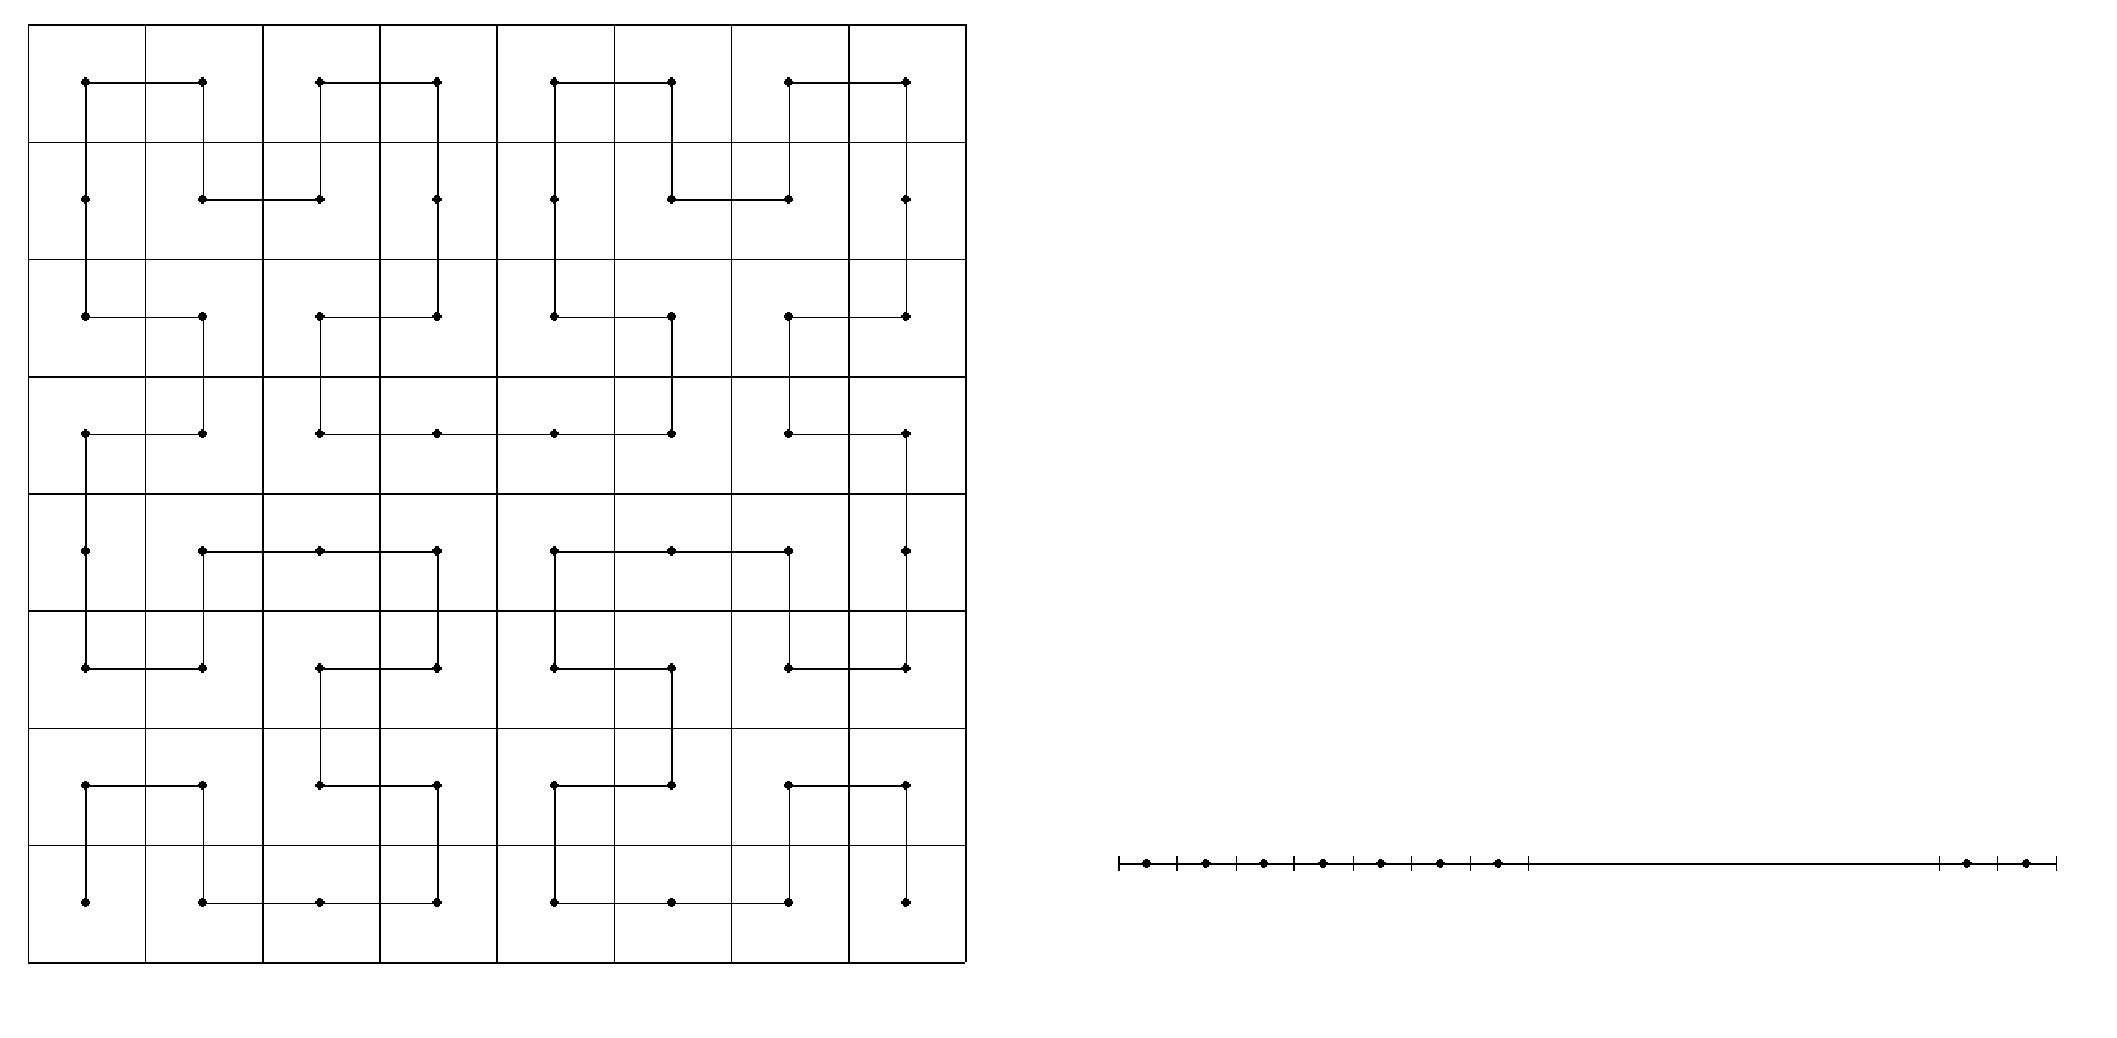
\includegraphics[width=0.85\textwidth]{pictures/peanoC.eps}
    \caption{A Peano curve approximation for the third density level}
    \label{fig:peanoC}
\end{figure}

\par
The computational scheme obtained as a result of the dimensionality reduction consists of the following
(see Figure \ref{fig:peanoCUsage}):
\begin{itemize}
  \item The optimization algorithm performs the minimization of the reduced one-dimensional
  function \(\varphi(y(x))\) from (\ref{eq:oneDimTask}),
  \item After determining the next trial point \(x\), a multidimensional image \(y\) is calculated by using the
mapping \(y(x)\),
  \item The value of the initial multidimensional function \(\varphi(y)\) is calculated at the point \(y\in D\),
  \item The calculated value \(z=\varphi(y)\) is used further as the value of the reduced one-dimensional function \(\varphi(y(x))\) at the point \(x\).
\end{itemize}

\begin{figure}
    \centering
    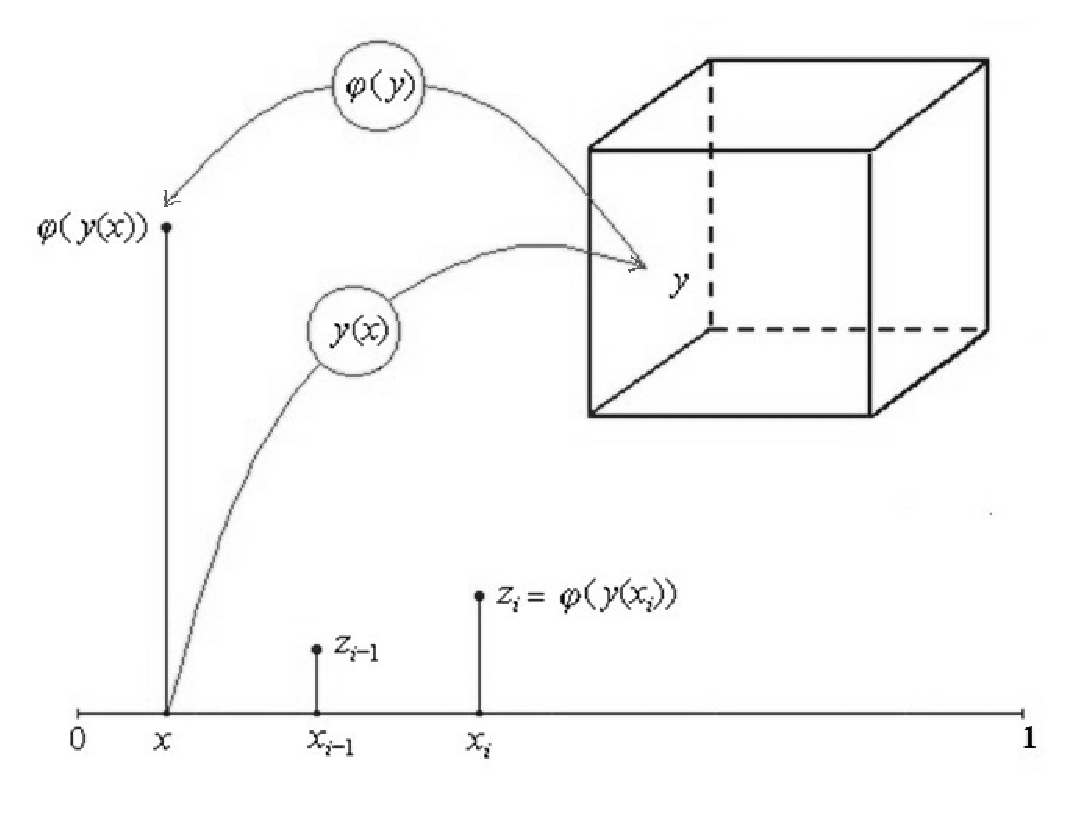
\includegraphics[width=0.55\textwidth]{pictures/peanoCUsage.eps}
    \caption{The computational scheme for obtaining the value of the reduced one-dimensional function \(\varphi(y(x))\)}
    \label{fig:peanoCUsage}
\end{figure}

\section{Parallel Computations for Solving Global Optimization Problems}
\label{sec:parallel}
Let us consider the parallelization approaches used widely in the theoretical and
practical applications of parallel computing within the context of global optimization problems:
\begin{itemize}
  \item The distribution of the search domain \(D\) among the available computational units (data parallelization scheme). This approach is insufficient in the case of optimization problems since in such computations the subdomain, which contain the sought global minimum, will only be processed by one processor, and, therefore, all the remaining processors would perform the excess computations.
  \item The parallelization of the optimization algorithms (task parallelization scheme). This approach is also insufficient since the direct computational costs for executing the optimization algorithms are relatively low (the majority of computations are represented by the calculations of the optimized function values due to the initial assumption of considerable computational costs of such calculations).
  \item The parallelization of the computations executed in order to obtain the values of the optimized function. This approach is applicable since the most time-consuming part of the global optimization will be parallelized. However, this method is not featured by the generality (the development of parallelization methods is to be performed every time from the very beginning while solving each particular optimization problem).
\end{itemize}
\par
Within the framework of the information-statistical theory, a general parallelization
approach for solving the global optimization problems has been proposed \cite{stronginGergelBarkalovParGO}, \cite{strSergGO} --- \textit{the parallel computations are provided by means of simultaneous computing the values of the
minimized function \(\varphi(y)\) at several different points within the search domain \(D\)}.
This approach provides the parallelization for the most time-consuming part of the optimization computations.
\par
The global optimization algorithms implemented in Globalizer will be described step-by-step.
In Subsection \ref{subsec:corepar}, the core serial Multidimensional Algorithm of Global
Search (MAGS) is presented. In Subsection \ref{subsec:sharedpar}, a parallel generalization
of the MAGS algorithm for the parallel computations on the multiprocessor computational
nodes with shared memory is described. In Subsection \ref{subsec:distribpar}, the scheme
for the parallel computations on the high-performance computational systems with distributed memory is given.

\subsection{Core Multidimensional Algorithm of Global Search}
\label{subsec:corepar}
The information-statistical theory of global optimization formulated in \cite{strongin1978}, \cite{strSergGO} has
served as a basis for the development of a large number of efficient multiextremal optimization
methods \cite{barkalovGergel2014}, \cite{gergel1996}, \cite{gergel1997}, \cite{grishaginStrongin1984}, \cite{Pizzuti}, \cite{sergeyev1995}, \cite{sergeyev1999}, \cite{sergeyevGrishagin2001}, \cite{sergeyevStronginLera2013}, \cite{Famularo2001}.
\par
The optimization methods applied in Globalizer are based on the MAGS method, which can be presented as follows --- see \cite{strongin1978}, \cite{strSergGO}.
\par
Let us introduce a simpler notation for the optimization problem being solved
\begin{equation}
\label{eq:oneDimFunc}
f(x) = \varphi(y(x)):x\in [0,1].
\end{equation}
\par
The initial iteration of the algorithm is performed at an arbitrary point \mbox{\(x^1\in(0,1)\)}.
Then, let us suppose that \(k\), \(k\ge 1\), optimization iterations have been completed already.
The selection of the trial point \(x^{k+1}\) for the next iteration is performed according to the following rules.
\par
\textit{Rule 1}. Renumber the points of the preceding trials by the lower indices in order of increasing value of coordinates
\begin{equation}
  \label{step1}
0=x_0<x_1<...<x_{k+1}=1,
\end{equation}
the points \(x_0\), \(x_k\) were introduced additionally for the convenience of further
explanation, the values of the minimized function \(z_0\), \(z_k\) at these points are undefined.
\par
\textit{Rule 2}. Compute current estimate of the H{\"o}lder constant \(H\) from (\ref{eq:holder})
\begin{equation} \label{step2}
M=\max_{1\leq i\leq k}\frac{|z_i-z_{i-1}|}{\rho_i}, \;
m = \left\{
   \begin{array}{lr}
     rM, & M > 0,\\
     1, & M = 0,
   \end{array}
  \right.
\end{equation}
as the maximum of the relative differences of the minimized function values on the
set of previously executed trial points \(x_i,1\leq i\leq k\) from (\ref{step1}).
Hereafter, \(\rho_i=(x_i-x_{i-1})^\frac{1}{N},1\leq i\leq k+1\). The
constant \(r\), \(r>1\), is the reliability parameter of the algorithm.
\par
\textit{Rule 3}. Compute the characteristics \(R(i)\) for each interval \((x_{i-1},x_i),1\leq i\leq k+1\), where
\[
R(i)=2\rho_i-4\frac{z_i}{m},\quad i=1,
\]
\begin{equation} \label{step3}
R(i)=\rho_i+\frac{(z_i-z_{i-1})^2}{m^2\rho_i}-2\frac{z_i+z_{i-1}}{m},\quad 1<i<k+1, \\
\end{equation}
\[
R(i)=2\rho_{i}-4\frac{z_{i-1}}{m},\quad i=k+1.
\]

\par
\textit{Rule 4}. Determine the interval with the maximum characteristic
\begin{equation} \label{step4}
R(t)=\max_{1\leq i \leq k+1}R(i).
\end{equation}
\par
\textit{Rule 5}. Execute a new trial at the point \(x^{k+1}\) located within the interval
with the maximum characteristic from (\ref{step4})
\begin{equation} \label{step5}
  x^{k+1}=\frac{x_t+x_{t-1}}{2}-\mathrm{sign}(z_{t}-z_{t-1})\frac{1}{2r}\left[\frac{r|z_{t}-z_{t-1}|}{m}\right]^N,\; \textrm{ if } 1<t<k+1,
\end{equation}
\[
  x^{k+1}=\frac{x_t+x_{t-1}}{2},\; \textrm{ if } t=1 \textrm{ or } t=k+1.
\]

\par
The stopping condition, which terminated the trials, is defined by the inequality
\begin{equation}
  \label{eq:stop_1}
\rho_t<\varepsilon
\end{equation}
for the interval with the maximum characteristic from (\ref{step4}) and \(\varepsilon >0\) is the predefined
accuracy of the optimization problem solution. If the stopping condition is not satisfied,
the index \(k\) is incremented by 1, and the new global optimization iteration is executed.
\par
In order to explain the algorithm presented above, let us note the following.
The characteristics \(R(i), 1\leq i\leq k+1\), calculated according to (\ref{step3}) could
be interpreted as some measures of importance of the intervals with respect to the
expected location of the global minimum point. Thus, the rules (\ref{step4}) and (\ref{step5}) for selecting
the interval for executing the next trial become more clear --- the point of every next
global optimization iteration is selected within the interval, where the global minimum
point can be found most likely.
\par
The convergence conditions of the described algorithm are given, for example, in \cite{strSergGO}.

\subsection{Parallel Computations for Systems with Shared Memory}
\label{subsec:sharedpar}
Modern supercomputer computational systems consist of plenty of computational nodes,
which include several multicore processors. In this case, random access memory
in the computational nodes is shared --- the content of any memory location can be read
(written) by any computational core at any arbitrary moment. In most cases, shared memory is
uniform --- the time characteristics for accessing the memory are the same for all
computational cores and for all memory locations.
\par
The following approach can be applied to provide the parallel computations with the MAGS method.
As it was mentioned above, the characteristics \(R(i),1\leq i\leq k+1\) calculated
according to (\ref{step3}) can be interpreted as some measures of importance of the
intervals with respect to the expected location of the global minimum point.
Following this understanding, every next global optimization iteration is executed within
the most important interval with the maximum characteristic. As a result, it becomes
evident how to select the other intervals for simultaneous computations of the minimized
function values at several different points within the search domain --- these ones
should be the intervals with the next magnitudes of characteristics.
\par
The computational scheme of the Parallel Multidimensional Algorithm of Global Search (PMAGS)
for the computational systems with shared memory can be developed based on the approach
described above. This scheme is almost identical to the MAGS one --- the differences
consist just in the following set of rules.
\par
\textit{Rule 4\'}. Arrange the characteristics of the intervals computed according to (\ref{step3}) in the decreasing order
\begin{equation}
\label{step4par}
R(t_1)\geq R(t_2)\geq \dots \geq R(t_{k})\geq R(t_{k+1})
\end{equation}
and select \(p\) intervals with the indices \(t_j,1\leq j\leq p\), with the maximum
values of characteristics (\(p\) is the number of processors/cores used for the parallel computations).
\par
\textit{Rule 5\'}. Execute new trials at the points \(x^{k+j},1\leq j\leq p\) located
in the intervals with the maximum characteristics from (\ref{step4par})

\begin{equation} \label{step5par}
x^{k+j}=\frac{x_{t_j}+x_{t_j-1}}{2}-\mathrm{sign}(z_{t_j}-z_{t_j-1})\frac{1}{2r}\left[\frac{r|z_{t_j}-z_{t_j-1}|}{m}\right]^N,\; \textrm{ if } 1<t_j<k+1,
\end{equation}
\[
x^{k+j}=\frac{x_{t_j}+x_{t_j-1}}{2},\; \textrm{ if } t_j=1 \textrm{ or } t_j=k+1.
\]
\par
The stopping condition (\ref{eq:stop_1}) should be checked for all intervals from (\ref{step4par}),
where the scheduled trials are executed
\begin{equation}
  \label{eq:stop}
\rho_{t_j}<\varepsilon,1\leq j\leq p.
\end{equation}
If the stopping condition is satisfied at least for one interval \(t_j, 1\le j\le p\), the calculations
are terminated. Otherwise, the index \(k\) is incremented by \(p\), and new global optimization iteration is executed.
\par
The convergence conditions for the developed parallel algorithm are considered
in \cite{stronginGergelBarkalovParGO}, \cite{strSergGO}. Thus, in particular, when the convergence conditions are
satisfied, the parallel computations are non-redundant as compared to the serial method
when using up to \(2^N\) processors/cores (\(N\) is the dimensionality of the global optimization problem).

\subsection{Parallel Computations for Systems with Distributed Memory}
\label{subsec:distribpar}
The next level of parallel computations on the high-performance computational systems
consists in using several computational nodes. In this case, each computational node has
its own separate memory and the interaction between different nodes can be provided by
means of data transfer via the computer communication network.
\par
To provide parallel computations on high-performance computational systems with the distributed memory, it is proposed to use a set of mappings
\begin{equation}
  \label{eq:maps}
Y_s(x)=\{y^1(x),\dots,y^s(x)\}
\end{equation}
instead of applying a single Peano curve \(y(x)\) --- see, for instance,
\cite{strongin1992}, \cite{stronginGergelBarkalovParGO}, \cite{strSergGO}.
In order to construct the set \(Y_s(x)\), several different approaches can be applied.
Thus, for example, in \cite{strongin1992} each mapping \(y^i(x)\) from \(Y_s(x)\) is constructed
as the result of some shift along the main diagonal of the hypercube \(D\). This way,
the set of the constructed Peano curves enables the close prototypes \(x'\), \(x''\)
to be obtained from the interval \([0, 1]\) for any close multidimensional images
\(y'\), \(y''\) from \(D\) differing in one coordinate only.
\par
Some other methods for constructing the multiple mappings were considered in \cite{stronginGergelBarkalovParGO}.
\par
The set of mappings \(Y_s(x)\) from (\ref{eq:maps}) generates \(s\) information-linked one-\linebreak
dimensional problems (\ref{eq:oneDimTask}):
\begin{equation}
  \label{eq:oneDimProblemSerie}
  \varphi(y^l(x^*))=\min\{\varphi(y^l(x)):x\in [0,1]\},1\leq l\leq s.
\end{equation}
\par
It is important to note that the family of the one-dimensional problems
$\varphi(y^l(x))$, $1 \leq l \leq s$ obtained as a result of the dimensionality
reduction is an information-linked one --- the function values computed for any
problem \(\varphi(y^l(x))\) from the family (\ref{eq:oneDimProblemSerie}) can be used for all rest problems of this family.
\par
The information compatibility of the optimization problems from the family (\ref{eq:oneDimProblemSerie})
allows executing the parallel computations in the following way. Each particular
problem can be solved by a separate processor of the computational system; the exchange
of search information between the processors should be performed during the computations.
As a result, a unified approach for the parallel computations on the high-performance
computational systems with distributed and shared memory can be developed. This method consists in the following.
\begin{enumerate}
  \item The family of the reduced one-dimensional information-linked optimization
  problems (\ref{eq:oneDimProblemSerie}) is distributed among the computational nodes of the multi-node computational system.
  \item Each optimization problem from the family (\ref{eq:oneDimProblemSerie}) is solved on the
  corresponding computational node using the PMAGS method (described above in Subsection \ref{subsec:sharedpar})
  supplemented by the following rules of the information interaction.
  \begin{enumerate}
    \item Prior to beginning new trial at any point \(x'\in [0,1]\) for any problem \(\varphi(y^l(x)),1\leq l\leq s\), the following should be performed:
    \begin{itemize}
      \item compute the image \(y'\in D\) for the point \(x'\in [0, 1]\) according to the mapping \(y^l(x)\),
      \item determine  the preimages\footnote{All preimages have the same
      image \(y'\); the preimages are calculated by the inverse mappings \((y^i)^{-1}\), \(1\le i\le s\);
      the number of the preimages coincides with the number of the mappings.}
      \begin{displaymath}
        x_i':y'=y^i(x'),1\le i\le s,
      \end{displaymath}
      in accordance with the set of mappings \(y^l(x), 1\le l\le s\) for each problem from the family (\ref{eq:oneDimProblemSerie}),
      \item send the prototypes \(x_i',1\leq i\leq s\) to all computational nodes in order
      to exclude the repeated selection of the intervals, which the prototypes fall in,
      for using these ones to determine the points of new trials. To perform the data transfer,
      a queue can be created at each computational node for sending the trial points and
      receiving the minimized function values at these points.
    \end{itemize}
    \item After completing any trial for any problem \(\varphi(y_l(x)),1\leq l\leq s\),
    at any point \(x'\in[0,1]\), it is necessary:
    \begin{itemize}
      \item to determine all prototypes \(x_i',1\leq i\leq s\) for the point of the
      completed trial for each problem from the family (\ref{eq:oneDimProblemSerie}),
      \item to send the prototypes \(x_i',1\leq i\leq s\) and the result of the trial
      \(z'=\varphi(y_l(x'))\) to all computational nodes to include the obtained data into
      the search information processed according to the rules of the parallel global optimization algorithm.
    \end{itemize}
    \item Prior to starting the next global optimization iteration, the algorithm
    should check the queue of the received data; if there are any data in the queue,
    these should be included into the search information. The MAGS algorithm uses these
    accumulated data for the adaptive computing of the optimization iteration points (see Section \ref{subsec:corepar}).
\end{enumerate}
\end{enumerate}
\par
The possibility of asynchronous data transfer (the computational nodes process the obtained
data after receiving only) is an important feature of the proposed parallel computation scheme.
In addition, there is no any selected managing node within this scheme. The number of
computational nodes can vary during the global optimization, and excluding any node does not result
in the loss of the sought global minimum of the minimized multiextremal function.
\par
This computational scheme generates the Generalized Parallel Multidimensional Algorithm of
Global Search (GPMAGS) for high-performance computational systems, which may include many
multiprocessor (multicore) computational nodes with distributed memory as well as the
computational accelerators based on Intel Xeon Phi processors and on the general purpose graphic processors (GPUs).
\par
Additional information on such parallel computation schemes can be found in \cite{gergelSidorov2015}.

\section{Globalizer System Architecture}
\label{sec:arch}
Globalizer expands the family of the global optimization software systems developed
by the authors during the past several years. One of the first developments was the
SYMOP multiextremal optimization system \cite{gergel1993}, which has been applied for solving
many optimization problems. The ExaMin system \cite{barkalovGergel2015}, \cite{barkalovGergelLebedev2015},
\cite{barkalovGergelLebedevSysoev2015}, \cite{gergelLebedev2015} was developed
and used to investigate various parallel algorithms for solving the global
optimization problems on the high-performance computational systems.

\begin{figure}
    \centering
    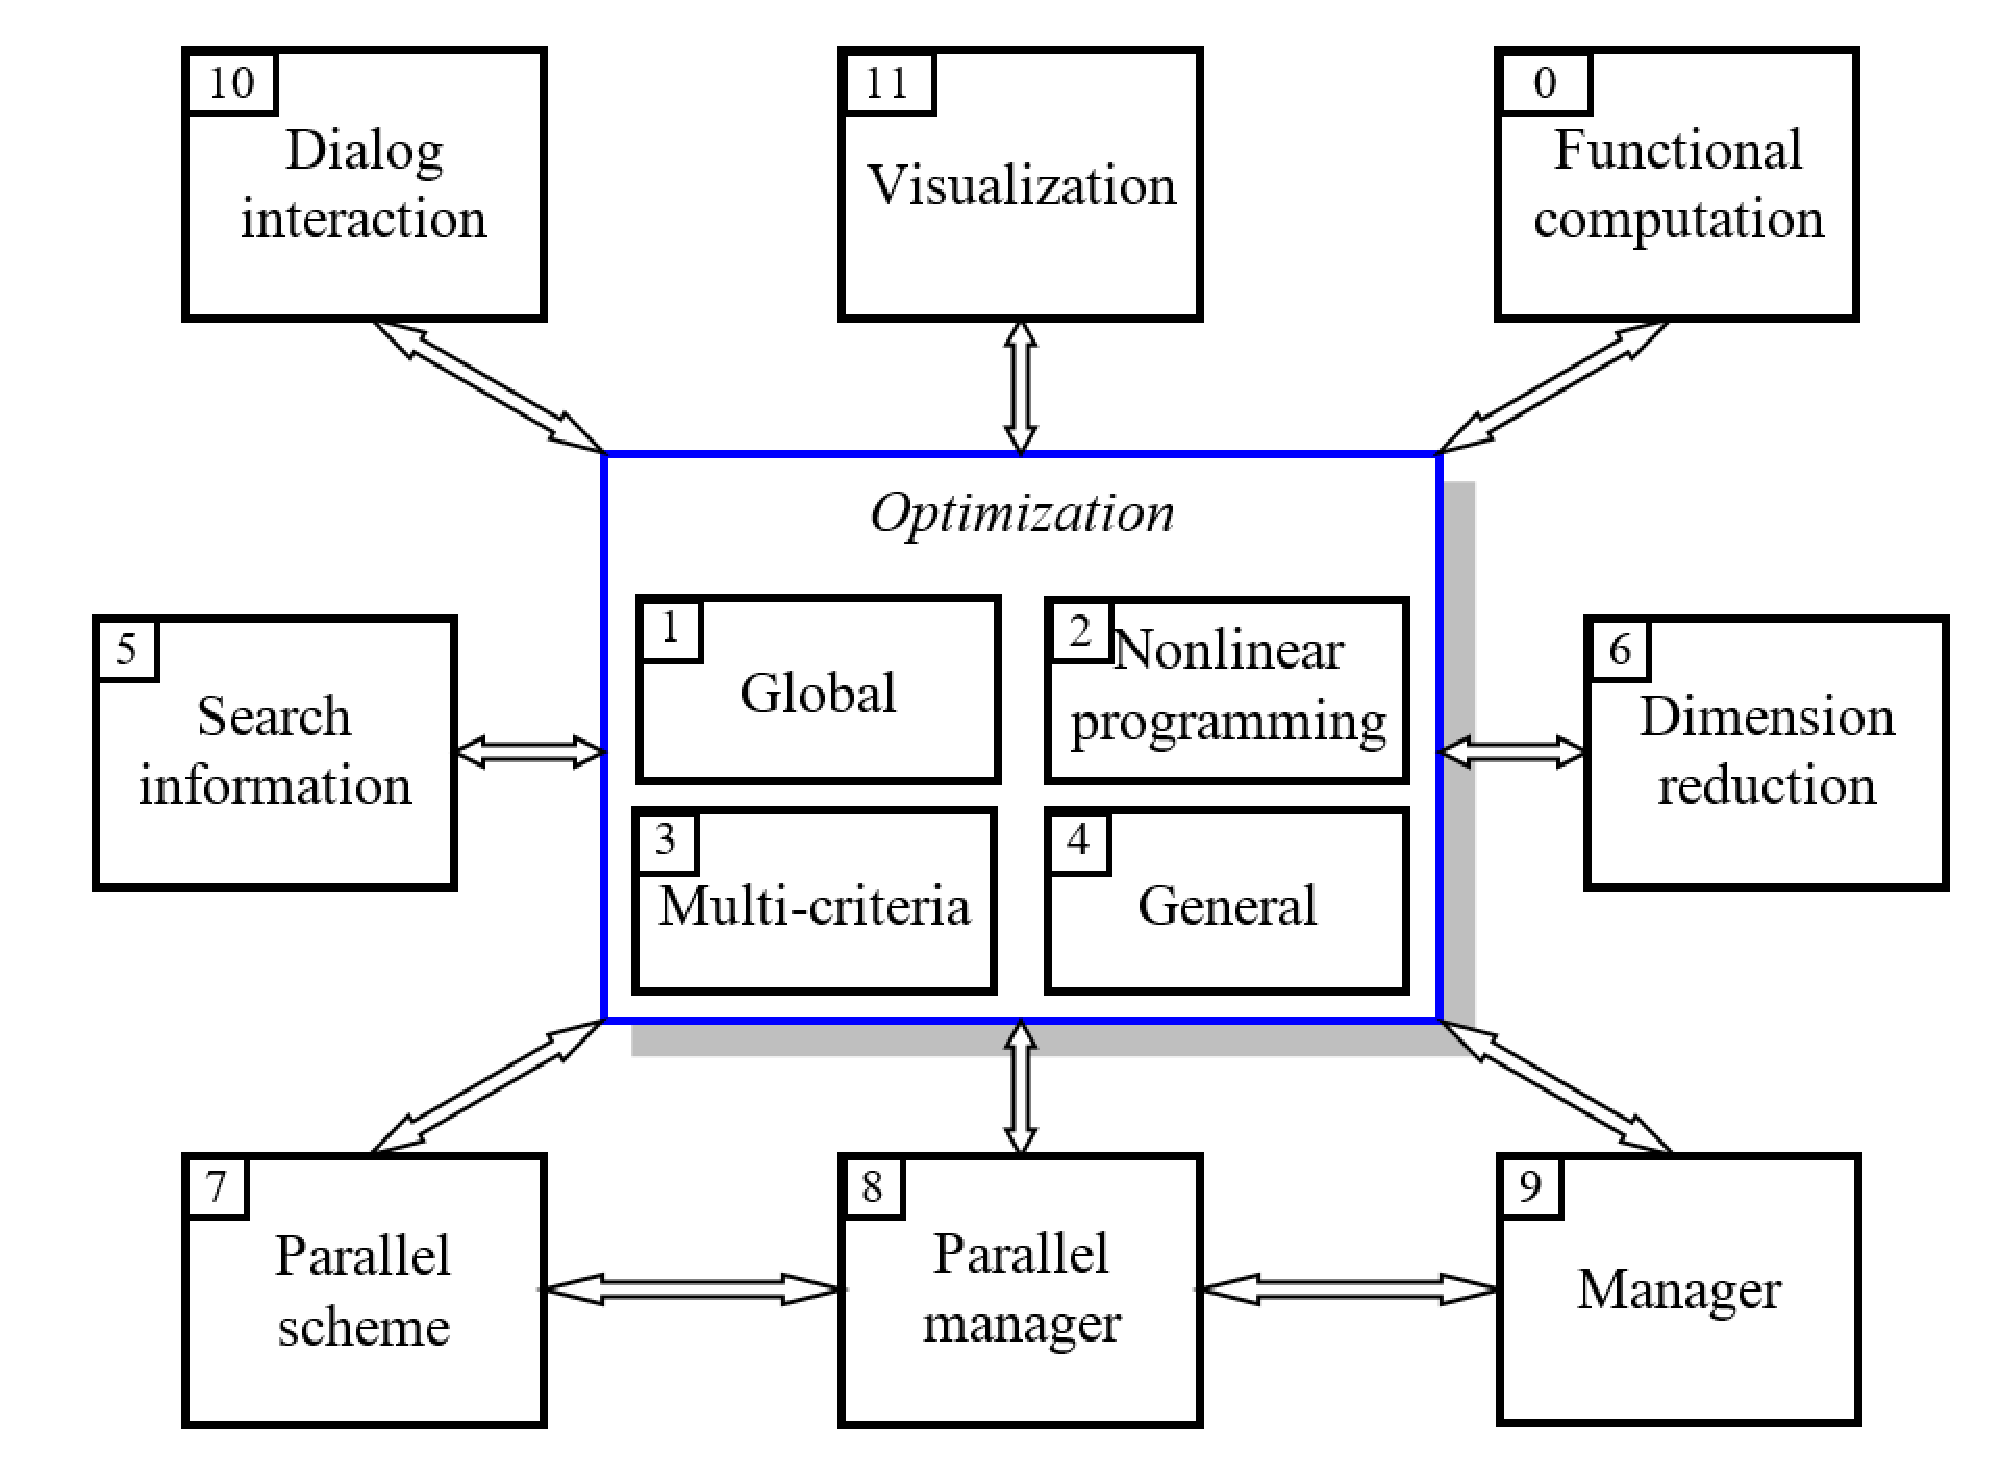
\includegraphics[width=0.75\textwidth]{pictures/globalizerScheme.eps}
    \caption{The architecture of the Globalizer system}
    \label{fig:globalizerScheme}
\end{figure}

\par
The architecture of the Globalizer system is presented in Figure \ref{fig:globalizerScheme}.
The system components are:
\begin{itemize}
  \item Block 0 consists of the procedures for computing the function values
  (criteria and constraints) of the optimization problem being solved; it is an external
  block with a predefined interface with respect to the Globalizer system and is provided by the user.
  \item Blocks 1-4 form the optimization subsystem and solve the global optimization
  problems (Block 1), nonlinear programming ones (Block 2), multicriterial optimization problems
  (Block 3), and general decision making problems (Block 4). The interaction between these
  components is organized in a hierarchical order --- the decision making problems are
  solved using the multicriterial optimization block, which, in turn, uses the nonlinear programming block, and so on.
  \item Block 5 is a subsystem for accumulating and processing the search information; it is one of the main subsystems – the size of search information may appear to be quite large and the efficiency of the global optimization methods depends on how completely the available search data are utilized.
  \item Block 6 contains the dimensionality reduction procedures based on the Peano space-filling curves; the reduced (one-dimensional) optimization problems are solved by the optimization blocks. This block also provides the interaction between the optimization blocks and the multidimensional optimization problem being solved.
  \item Block 7 provides tuning the parallel computation schemes in the Globalizer system subject to the employed computational system architecture (the number of the computational cores, the availability of shared and/or distributed memory, the availability of computational accelerators, etc.) and the applied global optimization methods.
  \item Block 8 is responsible for managing the parallel processes when performing the global optimization (determining the optimal configuration of parallel processes, distributing the processes between the computational units, balancing the computational loads, etc.).
  \item Block 9 is a managing subsystem, which controls the parallel computations when solving the global optimization problems.
  \item Block 10 provides the dialog interaction with the users for stating the optimization problem, adjusting the system parameters (if necessary), and visualizing and presenting the global optimization results.
  \item Block 11 is a set of tools for visualizing and presenting the global optimization results; the availability of the tools for visual demonstration of the computational results enables the user to perform an efficient control over the global optimization process.
\end{itemize}
\par
The Globalizer system comes in two different versions:
\begin{itemize}
  \item Globalizer Pro is a research version for making various large-scale numerical experiments on the high-performance computational systems to investigate the new parallel global optimization methods being developed.
  \item Globalizer Lite is a limited version for solving the global optimization problems with a medium complexity level, and is accessible for free usage.
\end{itemize}

\section{Results of Numerical Experiments}
\label{sec:experiments}
The numerical experiments were carried out using the Lobachevsky supercomputer at
the State University of Nizhni Novgorod (the operation system – CentOS 6.4, the
supercomputer management system – SLURM). Each supercomputer node had 2 Intel Sandy Bridge
E5-2660 processors, 2.2 GHz, with 64 GB RAM. Each processor had 8 cores (i. e. total
16 CPU cores were available at each node). In order to generate the executable program code, the Intel C++ 14.0.2 compiler was used.
\par
A number of computational nodes had Intel Xeon Phi 5110P processors, each containing 60 cores
(total 240 threads). In addition, the supercomputer included the computational nodes equipped
with two NVIDIA Kepler K20X GPUs, each providing 14 stream multiprocessors (total 2688 CUDA-cores). In order to generate the executable code, the CUDA Toolkit 6.0 was used.
\par
In the performed experiments the optimization problems generated by the GKLS-generator
\cite{gavianoKvasovLeraSergeev2003} were used. This generator allows obtaining the multiextremal optimization
problems with \textit{a priori} known properties: the number of local minima, the sizes of the attractors of these ones, the global minimum point, the function value at this point, etc. In order to simulate the computational costs that are inherent in the applied optimization problems, in all experiments computing the objective function values was intentionally complicated by the auxiliary computations not altering the values of the function and the position of its minima.
\par
In all the executed experiments, 100 global optimization problems generated randomly by the GKLS-generator were solved. The results of experiments were averaged over the number of the solved optimization problems.

\subsection{Comparison with over methods}
The results of numerical comparison of three serial algorithms --- DIRECT
\cite{Jones}, DIRECT\textit{l} \cite{Gablonsky}, and MAGS from Section \ref{subsec:corepar} --- are presented below.

The numerical comparison was carried out by using the function classes Simple and Hard
of the dimensions 4 and 5. The results of numerical experiments for DIRECT and
DIRECT\textit{l} are taken from \cite{sergeyevKvasov2006}. According to \cite{sergeyevKvasov2006}, the global minimizer \(y^*\)
was considered to be found if the algorithm generated a trial point \(y^k\) inside
a hyperinterval with a vertex \(y^*\) and
\begin{displaymath}
    |y^k(i)-y^*(i)|\le \sqrt[N]{\Delta}(b(i)-a(i)), i\le i\le N,
\end{displaymath}
where \(N\) is the problem dimensionality, $a$ and $b$ are the borders of the search domain \(D\)
\footnote{In the case of MAGS, the stop condition was different slightly --- the
global minimizer \(y^*\) was considered to be found, if MAGS generates a trial
point \(y^k\)  in the \(\delta\)-vicinity of the global minimum, i. e. \(||y^k-y^*||\le\delta\).
The size of the vicinity was selected  as \(\delta=\left\|b-a\right\|\sqrt[N]{\Delta}\).}.

The values of the parameter \(\Delta = 10^{-6}\) at \(N = 4\) and \(\Delta = 10^{-7}\)
at \(N = 5\) were used. When using MAGS, the reliability parameter was selected as
follows: \(r = 4.5\) for the Simple class and \(r = 5.6\) for the Hard class.
The density level parameter of the Peano curve approximation was fixed as \(m = 10\).

The averaged numbers of iterations $k_{av}$ executed by the global optimization methods
for solving the optimization problems are shown in Table \ref{tab:3}. The symbol ''$>$''
denotes the situation, when not all problems of the class are solved by the optimization
method. This means that the algorithm was stopped as the maximum allowed number of
iterations $K_{max}$ was achieved. In this case, the value $K_{max}= 10^6$  was used to
calculate the averaged number of iterations $k_{av}$ that corresponds to the lower estimate
of this averaged value. The number of the unsolved problems is specified in the brackets.

\begin{table}
  \caption{Averaged number of executed iterations of the compared global optimization methods}
  \label{tab:3}
  \center
  \begin{tabular}{lllll}
    \hline\noalign{\smallskip}
     $N$ & Problem class & DIRECT & DIRECT\textit{l} & MAGS \\
    \noalign{\smallskip} \hline \noalign{\smallskip}
      4 &	\textit{Simple}	& $>$47282(4) &	18983 &	11953 \\
        & \textit{Hard} &	$>$95708(7) &	68754 &	25263 \\
      5	& \textit{Simple} &	$>$16057(1) &	16758 &	15920 \\
        & \textit{Hard} &	$>$217215(16) &	$>$269064(4) & $>$148342(4) \\
    \noalign{\smallskip}\hline
  \end{tabular}
\end{table}

Table \ref{tab:3} demonstrates that MAGS overcomes the DIRECT and DIRECT\textit{l} methods
on all classes of problems in terms of the averaged number of iterations.
In the 5-Hard class, all three methods failed to solve some problems: DIRECT did not
solve 16 problems, DIRECT\textit{l} and MAGS --- 4 problems each.

\subsection{Parallel Computations Using Intel Xeon Phi processors}
As in the previous case, the numerical experiments were performed by using the Simple
and Hard function classes with the dimensions equal to 4 and 5. The values of the
parameter \(\Delta=10^{-6}\) at \(N=5\) and \(\Delta=10^{-7}\) at \(N=5\) were used.
When using the GPMAGS method, the values of the reliability parameter \(r=4.5\) was
selected for the Simple class and \(r=5.6\) was selected for the Hard class.

The results of the numerical experiments executed by using GPMAGS with Intel Xeon Phi processors are presented in Tables \ref{tab:4} and \ref{tab:5}.

In the first series of experiments, the serial computations using MAGS were executed.
The average numbers of iterations performed by the method for solving the series of optimization problems
for each class are shown in row I.

In the second series of experiments, the parallel computations were executed using the CPUs.
The achieved relative speedup in iterations is shown in row II; the speedup of the
parallel computations is shown relative to the serial computations \((p=1)\).

The final series of experiments was executed using Xeon Phi processors. The results
of these experiments are shown in row III. In this case, the speedup is
calculated relative to the results of the PMAGS method executed on the CPU using eight cores \((p=8)\).

\begin{table}
  \centering
  \caption{Averaged numbers of iterations executed by GPMAGS for solving the test optimization problems}
  \label{tab:4}
  \begin{tabular}{cccccccc}
    \cline{3-8}\noalign{\smallskip}
    \multicolumn{2}{c}{  } & \textit{p} & \multicolumn{2}{c}{$N=4$} & & \multicolumn{2}{c}{$N=5$}   \\
    \noalign{\smallskip} \cline{4-5} \cline{7-8}  \noalign{\smallskip}
    \multicolumn{2}{c}{  } & & \textit{Simple} & \textit{Hard} & & \textit{Simple} & \textit{Hard}  \\
    \noalign{\smallskip}\hline
    I &
    \parbox{0.25\textwidth}{
    \begin{center}
    \textbf{Serial trial computations}
    \end{center}		}
      & 1 & 11953 & 25263 & & 15920 & \(>\)148342 (4)  \\
    \hline \noalign{\smallskip}
II  & \textbf{Parallel computations}  %\multirow{3}{*}{}
  & 2 & 4762 & 11178 & & 13378 & 109075 \\
& on CPU & 4 & 2372 & 5972 & & 5203 & 51868 \\
&  & 8 & 1393 & 2874 & & 3773 & 51868 \\
    \noalign{\smallskip}\hline	\noalign{\smallskip}
III & \textbf{Parallel computations} %\multirow{3}{*}{}
  & 60  & 171 & 393 & & 382 & 3452  \\
& on Xeon Phi  & 120 & 85 & 182 & & 249 & 1306 \\
&  & 240 & 42 & 103 & & 97 & 381 \\

    \noalign{\smallskip}\hline
  \end{tabular}
\end{table}

\begin{table}
  \centering
  \caption{Speedup of parallel computations executed by GMAGS}
  \label{tab:5}
  \begin{tabular}{cccccccc}
    \cline{3-8}\noalign{\smallskip}
    \multicolumn{2}{c}{  } & \textit{p} & \multicolumn{2}{c}{$N=4$} & & \multicolumn{2}{c}{$N=5$}   \\
    \noalign{\smallskip} \cline{4-5} \cline{7-8}  \noalign{\smallskip}
    \multicolumn{2}{c}{  } & & \textit{Simple} & \textit{Hard} & & \textit{Simple} & \textit{Hard}  \\
    \noalign{\smallskip}\hline
    I &
    \parbox{0.25\textwidth}{
    \begin{center}
    \textbf{Serial trial computations.}\\ \textit{Average number} \\ \textit{of iterations}
    \end{center}		}
      & 1 & 11953 & 25263 & & 15920 & \(>\)148342 (4)  \\
    \hline \noalign{\smallskip}
II  & \textbf{Parallel computations}  %\multirow{3}{*}{}
  & 2 & 2.52 & 2.32 & & 1.21 & 1.41 \\
& of CPU. & 4 & 5.05 & 4.24 & & 3.13 & 2.92 \\
& \textit{Speedup} & 8 & 8.68 & 8.88 & & 4.24 & 6.66 \\
    \noalign{\smallskip}\hline	\noalign{\smallskip}
III & \textbf{Parallel computations} %\multirow{3}{*}{}
  & 60  & 8.18 & 7.37 & & 9.99 & 6.66  \\
&  of Xeon Phi. & 120 & 16.316 & 15.815 & & 15.215 & 17.317 \\
& \textit{Speedup} & 240 & 33.133 & 27.827 & & 38.838 & 59.359 \\

    \noalign{\smallskip}\hline
  \end{tabular}
\end{table}

\subsection{Parallel Computations Using General Purpose Graphic Processors}
In the first series of experiments, single graphic accelerator was used for solving 100
6-dimensional optimization problems. The reliability parameter \(r=4.5\) was selected.
\par
The averaged execution time using GPU was 10.78 sec whereas the averaged execution
time using all 16 CPU cores of the computational node was 53.8 sec; almost 5-fold improvement was observed.
\par
A larger scale computational experiment was carried out for the global optimization
problems with the dimensions of \(N = 8\) and \(N = 10\): total 12 nodes with 36 graphic
accelerators (three accelerators per the computational node) were employed (total 96768 CUDA-cores were used).
\par
The averaged execution time using the GPUs to solve the 8-dimensional problem was
405.6 sec that was 5.9 times less than the execution time for CPU. The averaged time
of solving the 10-dimensional problem was 2055.8 sec (in this case, the execution time for CPU
was not calculated because of the high complexity level of the required computations).

\section{Conclusions} \label{sec:concl}

In this paper, the Globalizer global optimization system for solving the time-consuming global optimization problems using a wide spectrum of high-performance computational systems (the systems with shared and distributed memory, the systems with NVIDIA graphic processors and Intel Xeon Phi coprocessors) was considered. The highly parallel computations were facilitated using various distinctive computational schemes: processing several optimization iterations simultaneously, reducing multidimensional optimization problems using multiple Peano space-filling curves, and the multi-stage computing based on nested block reduction schemes. The numerical experiments have confirmed the efficiency of the Globalizer system.

In future, it is planned to extend the Globalizer system for solving the multicriterial multiextremal multidimensional optimization problems with the nonlinear constraints. As a valuable part of further work, Globalizer would be used for solving the applied optimization problems from various application fields.
% You may incorporate your references as follows in your main tex file.
% Using BibTex is not recommended but can be handled.
%\bibliographystyle{plain}
%\bibliography{paper}

\begin{thebibliography}{10}

\bibitem{barkalovGergel2014}
\newblock K. A. Barkalov and V. P. Gergel,
\newblock Multilevel scheme of dimensionality reduction for parallel global search algorithms,
\newblock in \emph{Proceedings of the 1st International Conference on
  Engineering and Applied Sciences Optimization}, (2014), 2111--2124.

\bibitem{barkalovGergel2015}[10.1007/s10898-016-0411-y]
\newblock K. Barkalov and V. Gergel,
\newblock Parallel global optimization on GPU,
\newblock \emph{J. Glob. Optim.}, \textbf{66(1)} (2016), 3--20.

\bibitem{barkalovGergelLebedev2015}[10.1007/978-3-319-21909-7_31]
\newblock K. Barkalov, V. Gergel and I. Lebedev,
\newblock Use of XeonPhi coprocessor for solving global optimization problems,
\newblock \emph{LNCS}, \textbf{9251} (2015), 307--318.

\bibitem{barkalovGergelLebedevSysoev2015}
\newblock K. Barkalov, V. Gergel, I. Lebedev, A. Sysoev, %http://ceur-ws.org/Vol-1482/
\newblock Solving the global optimization problems on heterogeneous cluster systems,
\newblock in \emph{CEUR Workshop Proceedings}, \textbf{1482} (2015), 411--419.
%\newblock (In Russian).

\bibitem{Barkalov2013}[10.1007/978-3-642-39958-9_14]
\newblock K. Barkalov, A. Polovinkin, I. Meyerov, S. Sidorov, N. Zolotykh,
\newblock SVM regression parameters optimization using parallel global search algorithm,
\newblock \emph{LNCS}, \textbf{7979} (2013), 154--166.

\bibitem{bussieckMeeraus2004}[10.1007/978-1-4613-0215-5_8]
\newblock M. R. Bussieck and A. Meeraus,
\newblock General algebraic modeling system (GAMS), in \emph{Modeling Languages in Mathematical Optimization} (ed. J. Kallrath),
\newblock Springer (2004), 137--157.

\bibitem{censorZeniosParGO}
\newblock Y. Censor and S. A. Zenios,
\newblock \emph{Parallel optimization: theory, algorithms, and applications},
\newblock Oxford University Press (1998).

\bibitem{ciegisHentyParGO}[10.1007/978-0-387-09707-7]
\newblock R. \v Ciegis, D. Henty, B. K\aa gstr\"om and J. \v Zilinskas,
\newblock \emph{Parallel scientific computing and optimization: advances and applications},
\newblock Springer (2009).

\bibitem{iosoDescription}
\newblock I. N. Egorov, G. V. Kretinin, I. A. Leshchenko and S. V. Kuptzov,
\newblock IOSO optimization toolkit --- novel software to create better design,
\newblock in \emph{9th AIAA/ISSMO Symposium on Multidisciplinary Analysis and Optimization}, 2002.
\newblock Available from \url{http://www.iosotech.com/text/2002\_4329.pdf}.

\bibitem{Famularo1999}[10.1016/S0005-1098(99)00058-8]
\newblock D. Famularo, P. Pugliese and Y. D. Sergeyev,
\newblock A global optimization technique for checking parametric robustness,
\newblock \emph{Automatica}, \textbf{35} (1999), 1605--1611.

\bibitem{fasanoPinter2013}[10.1007/978-1-4614-4469-5]
\newblock G. Fasano and J. D. Pint\'er,
\newblock \emph{Modeling and optimization in space engineering},
\newblock Springer, 2013.

\bibitem{floudasPardalosGOState}[10.1007/978-1-4613-3437-8]
\newblock C. A. Floudas and M. P. Pardalos,
\newblock \emph{State of the art in global optimization: computational methods and applications},
\newblock Kluwer Academic Publishers, Dordrecht (1996).

\bibitem{floudasPardGO}[10.1007/s10898-008-9332-8]
\newblock C. A. Floudas and M. P. Pardalos,
\newblock \emph{Recent advances in global optimization},
\newblock Princeton University Press (2016).

\bibitem{Gablonsky}[10.1023/A:1017930332101]
\newblock J. M. Gablonsky and C. T. Kelley,
\newblock A locally-biased form of the DIRECT algorithm,
\newblock \emph{J. Glob. Optim.}, \textbf{21(1)} (2001), 27--37.

\bibitem{gavianoKvasovLeraSergeev2003}[10.1145/962437.962444]
\newblock M. Gaviano, D. E. Kvasov, D. Lera and Y. D. Sergeev,
\newblock Software for generation of classes of test functions with known local and global minima for global optimization,
\newblock \emph{ACM Trans. Math. Software}, \textbf{29(4)} (2003), 469--480.

\bibitem{gergelLebedev2015}[10.1016/j.procs.2015.11.008]
\newblock V. Gergel and I. Lebedev,
\newblock Heterogeneous parallel computations for solving global optimization problems,
\newblock \emph{Procedia Comput. Sci.}, \textbf{66} (2015), 53--62.

\bibitem{gergel1993}
\newblock V. P. Gergel,
\newblock A software system for multi-extremal optimization,
\newblock \emph{Eur. J. Oper. Res.}, \textbf{65(3)} (1993), 305--313.

\bibitem{gergel1996}
\newblock V. P. Gergel,
\newblock A method for using derivatives in the minimization of multiextremum functions,
\newblock \emph{Comput. Math. Math. Phys.}, \textbf{36(6)} (1996), 729--742.

\bibitem{gergel1997}[10.1023/A:1008290629896]
\newblock V. P. Gergel,
\newblock A global optimization algorithm for multivariate functions with Lipschitzian first derivatives,
\newblock \emph{J. Glob. Optim.}, \textbf{10(3)} (1997), 257--281.

\bibitem{gergel2013}[doi:10.1016/j.procs.2013.05.164]
\newblock V. P. Gergel, et al.,
\newblock High performance computing in biomedical applications,
\newblock \emph{Procedia Computer Science}, \textbf{18} (2013), 10--19.

\bibitem{gergel2015}[10.15866/ireaco.v8i1.4935]
\newblock V. P. Gergel, et al.,
\newblock Recognition of surface defects of cold-rolling sheets based on method of localities,
\newblock \emph{International Review of Automatic Control }, \textbf{8(1)} (2015), 51--55.

\bibitem{gergelSidorov2015}[10.1007/978-3-319-21909-7_49]
\newblock V. P. Gergel and S. V. Sidorov,
\newblock A two-level parallel global search algorithm for solving computationally intensive multi-extremal optimization problems,
\newblock \emph{LNCS}, \textbf{9251} (2015), 505--515.

\bibitem{grishaginStrongin1984}
\newblock V. A. Grishagin and R. G. Strongin,
\newblock Optimization of multi-extremal functions subject to monotonically unimodal constraints,
\newblock \emph{Engineering Cybernetics}, \textbf{5} (1984), 117--122.

\bibitem{holmstromEdvall2004}[10.1007/978-1-4613-0215-5_19]
\newblock K. Holmström and M. M. Edvall,
\newblock The TOMLAB optimization environment,
\newblock \emph{Modeling Languages in Mathematical Optimization},
\newblock 369--376, Springer (2004).

\bibitem{horstTuyGO}[10.1007/978-3-662-03199-5]
\newblock R. Horst and H. Tuy,
\newblock \emph{Global optimization: deterministic approaches},
\newblock Springer-Verlag, Berlin (1990).

\bibitem{Jones}[10.1007/BF00941892]
\newblock D. R. Jones, C. D. Perttunen and B. E. Stuckman,
\newblock Lipschitzian optimization without the Lipschitz constant,
\newblock \emph{J. Optim. Theory Appl.}, \textbf{79(1)} (1993), 157--181.

\bibitem{kearfott2009}[10.1080/10556780802614051]
\newblock R. B. Kearfott,
\newblock GlobSol user guide,
\newblock \emph{Optim. Methods Softw.}, \textbf{24} (2009), 687--708.

\bibitem{Kvasov2015}[10.1016/j.advengsoft.2014.09.014]
\newblock D. E. Kvasov and Y. D. Sergeyev,
\newblock Deterministic approaches for solving practical black-box global optimization problems,
\newblock \emph{Adv. Eng. Softw.}, \textbf{80} (2015), 58--66.

\bibitem{Menniti}[10.1016/j.epsr.2007.10.009]
\newblock D. E. Kvasov, D. Menniti, A. Pinnarelli, Y. D. Sergeyev and N. Sorrentino,
\newblock Tuning fuzzy power-system stabilizers in multi-machine systems by global optimization algorithms based on efficient domain partitions,
\newblock \emph{Electric Power Systems Research}, \textbf{78(7)} (2008), 1217--1229.

\bibitem{Pizzuti}[10.1007/s00211-002-0419-8]
\newblock D. E. Kvasov, C. Pizzuti and Y. D. Sergeyev,
\newblock Local tuning and partition strategies for diagonal go methods,
\newblock \emph{Numerische Mathematik}, \textbf{94(1)} (2003), 93--106.

\bibitem{liberti2009}[10.1007/0-387-30528-9_8]
\newblock L. Liberti,
\newblock Writing global optimization software,
\newblock in \emph{Nonconvex Optimization and Its Applications }, \textbf{84}, 211--262,
\newblock Springer (2006).

\bibitem{linSchrage2009}[10.1080/10556780902753221]
\newblock Y. Lin and L. Schrage,
\newblock The global solver in the LINDO API,
\newblock \emph{Optim. Methods Softw.}, \textbf{24(4-5)} (2009), 657--668.

\bibitem{locatelliSchoenGO}[10.1137/1.9781611972672]
\newblock M. Locatelli and F. Schoen,
\newblock \emph{Global optimization: theory, algorithms and applications},
\newblock SIAM (2013).

\bibitem{luqueAlbaGA}[10.1007/978-3-642-22084-5]
\newblock G. Luque and E. Alba,
\newblock \emph{Parallel genetic algorithms. Theory and real world applications},
\newblock Springer-Verlag, Berlin (2011).

\bibitem{mongeauKarsentyRouze2000}[10.1080/10556780008805783]
\newblock M. Mongeau, H. Karsenty, V. Rouzé and J. B. Hiriart-Urruty,
\newblock Comparison of public-domain software for black box global optimization,
\newblock \emph{Optim. Methods Softw.}, \textbf{13} (2000), 203--226.

\bibitem{mullen2014}[10.18637/jss.v060.i06]
\newblock K. M. Mullen,
\newblock Continuous global optimization in R,
\newblock \emph{J. Stat. Softw.}, \textbf{60(6)} (2014).

\bibitem{pardalosZhigljavskyZilinskas2016}[10.1007/978-3-319-29975-4]
\newblock M. P. Pardalos, A. A. Zhigljavsky and J. \v Zilinskas,
\newblock \emph{Advances in stochastic and deterministic global optimization},
\newblock Springer (2016).

\bibitem{pinterGO}[10.1007/978-1-4757-2502-5]
\newblock J. D. Pint\'er,
\newblock \emph{Global optimization in action (Continuous and Lipschitz optimization: algorithms, implementations and applications)},
\newblock Kluwer Academic Publishers, Dordrecht (1996).

\bibitem{pinter2009}
\newblock J. D. Pint\'er,
\newblock Software development for global optimization,
\newblock \emph{Lectures on Global Optimization. Fields Institute Communications}, \textbf{55} (2009), 183--204.

\bibitem{riosSahinidis2013}[10.1007/s10898-012-9951-y]
\newblock L. M. Rios and N. V. Sahinidis,
\newblock Derivative-free optimization: a review of algorithms and comparison of software implementations,
\newblock \emph{J. Glob. Optim.}, \textbf{56} (2013), 1247--1293.

\bibitem{sahinidis1996}[10.1007/BF00138693]
\newblock N. V. Sahinidis,
\newblock BARON: A general purpose global optimization software package,
\newblock \emph{J. Glob. Optim.}, \textbf{8} (1996), 201--205.

\bibitem{sergeyev1995}[10.1137/0805041]
\newblock Y. D. Sergeyev,
\newblock An information global optimization algorithm with local tuning,
\newblock \emph{SIAM J. Optim.}, \textbf{5(4)} (1995), 858--870.

\bibitem{sergeyev1999}
\newblock Y. D. Sergeyev,
\newblock Multidimensional global optimization using the first derivatives,
\newblock \emph{Comput. Math. Math. Phys.}, \textbf{39(5)} (1999), 743--752,.

\bibitem{sergeyevKvasov2006}[	arXiv:1103.2056]
\newblock Y. D. Sergeyev, D. E. Kvasov,
\newblock Global search based on efficient diagonal partitions and a set of Lipschitz constants,
\newblock \emph{SIAM Journal on Optimization}, \textbf{16(3)} (2006), 910--937.

\bibitem{sergeyevGrishagin2001}[10.1023/A:1010185125012]
\newblock Y. D. Sergeyev and V. A. Grishagin,
\newblock Parallel asynchronous global search and the nested optimization scheme,
\newblock \emph{J. Comput. Anal. Appl.}, \textbf{3(2)} (2001), 123--145.

\bibitem{sergeyevStronginLera2013}[10.1007/978-1-4614-8042-6]
\newblock Y. D. Sergeyev, R. G. Strongin and D. Lera,
\newblock \emph{Introduction to global optimization exploiting space-filling curves},
\newblock Springer (2013).

\bibitem{Famularo2001}[10.1023/A:1012391611462]
\newblock Y. D. Sergeyev, D. Famularo and P. Pugliese,
\newblock Index branch-and-bound algorithm for Lipschitz univariate global optimization with multiextremal constraints,
\newblock \emph{J. Glob. Optim.}, \textbf{21(3)} (2001), 317--341.

\bibitem{strongin1978}
\newblock R. G. Strongin,
\newblock \emph{Numerical methods in multi-extremal problems (information-statistical algorithms)},
\newblock Moscow: Nauka, In Russian (1978).

\bibitem{strongin1992}[10.1007/BF00122428]
\newblock R. G. Strongin,
\newblock Algorithms for multi-extremal mathematical programming problems employing a set of joint space-filling curves,
\newblock \emph{J. Glob. Optim.}, \textbf{2(4)} (1992), 357--378.

\bibitem{stronginGergelBarkalovParGO}
\newblock R. G. Strongin, V. P. Gergel, V. A. Grishagin and K. A. Barkalov,
\newblock \emph{Parallel computations for global optimization problems},
\newblock Moscow State University (In Russian), Moscow (2013).

\bibitem{strSergGO}[10.1007/978-1-4615-4677-1]
\newblock R.G. Strongin and Y.D. Sergeyev,
\newblock \emph{Global optimization with non-convex constraints. Sequential and parallel algorithms},
\newblock Kluwer Academic Publishers, Dordrecht (2000).

\bibitem{zilinskTornGO}[10.1007/3-540-50871-6]
\newblock A. T\"orn and A. \v Zilinskas,
\newblock \emph{Global optimization},
\newblock Springer (1989).

\bibitem{venkataraman2009}
\newblock P. Venkataraman,
\newblock \emph{Applied optimization with MATLAB programming},
\newblock John Wiley \& Sons (2009).

\bibitem{zhigljavskyRandGO}[10.1007/978-94-011-3436-1]
\newblock A. A. Zhigljavsky,
\newblock \emph{Theory of global random search},
\newblock Kluwer Academic Publishers, Dordrecht (1991).

\end{thebibliography}

\medskip
% The data information below will be filled by AIMS editorial staff
Received xxxx 20xx; revised xxxx 20xx.
\medskip

\end{document}
